\chapter{コヒーレント状態を用いた通信}
次にコヒーレント状態を用いた通信について考える。
複素振幅αを持つ光の状態をコヒーレント状態と呼ぶ。コヒーレント状態$\alpha$は以下のような式で与えることができる。

\begin{equation}
|\alpha\rangle=\sum_nC_n|n\rangle
\end{equation}


ここでは、$\alpha$を実数として、コヒーレント状態 $\alpha$、$-\alpha$を用いて通信について考える。

この通信では、$0$に対して$-\alpha$を、$1$に対して$\alpha$を送信する。
受信者はホモダイン測定を行い、その測定値に対してしきい値処理をおこなって$0$または$1$出力する。


ホモダイン測定では、コヒーレント状態の複素振幅$\alpha=x+iy$の$x$成分を測定する。

    \begin{figure}[H]
        \centering   
        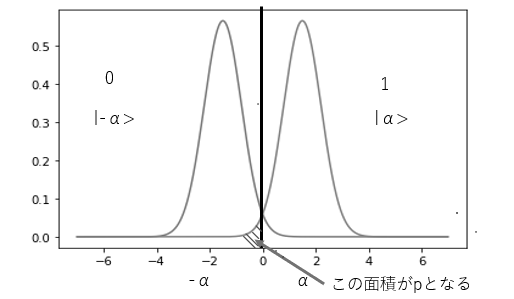
\includegraphics[width=1\textwidth]{img/Fig3.png}
        \caption[sample image (png)]{コヒーレント状態をホモダイン測定した場合の出力の確率分布}
        \label{Fig4_1}
    \end{figure}




\figref{Fig4_1}は、コヒーレント状態$\alpha$と$-\alpha$の測定値の確率分布のグラフを表している。この分布はそれぞれ分散$1/4$の正規分布となっている。
そして、閾値を$0$に設定し測定値が$0$より小さい場合は$0$、大きい場合は$1$を受信したと判断する。
したがって、この通信路は2元対称通信路となり、この面積が誤り確率$p$を表している。
したがって、この面積を計算すると通信容量を求めることが可能になる。


誤り確率$p$は、以下のような積分によって計算することができる。
$$
\int_{-\infty}^{x_0}f(x)dx
$$この積分は累積分布関数を用いて計算することができる。
累積分布関数はPythonを用いると以下のように書くことによって計算することができる。

\begin{lstlisting}[caption=累積分布関数]
p=norm.cdf(0,loc=x,scale=0.25)
\end{lstlisting}

また、通信容量は以下のように書いて計算することができる。

\begin{lstlisting}[caption=通信容量]
C=1+p*np.log(p)+(1-p)*np.log(1-p)
\end{lstlisting}


    \begin{figure}[H]
        \centering   
        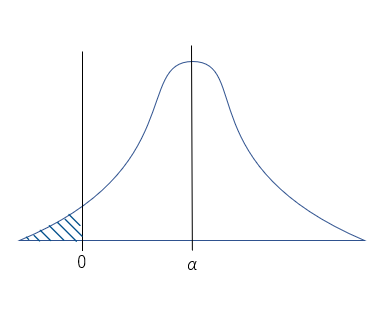
\includegraphics[width=0.7\textwidth]{img/Fig4.png}
         \caption[sample image (png)]{正規分布}
        \label{Fig4_2}
    \end{figure}

\figref{Fig4_2}はコヒーレント状態$|x\rangle$の測定値の確率分布のグラフをわかりやすくしたものである。


\begin{lstlisting}[caption=αの変化で変わる通信容量]
x=np.arange(0,5,0.01)
p=norm.cdf(0,loc=x,scale=0.25)
c=1+p*np.log(p)+(1-p)*np.log(1-p)
plt.plot(x,c)
\end{lstlisting}
\figref{Fig4_3}は、通信容量の計算の結果である。
信号$\alpha$と$-\alpha$を区別することが容易となるので誤り率$p$はほとんど$0$となる。
そのため\figref{Fig4_3}において、$\alpha$の値が大きくなると、通信容量$1$に近づいている。

    \begin{figure}[H]
        \centering   
        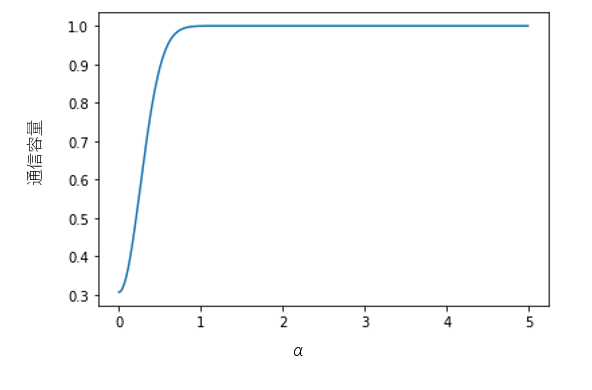
\includegraphics[width=0.7\textwidth]{img/Fig5.png}
        \caption[sample image (png)]{$\alpha$の変化で変わる通信容量}
        \label{Fig4_3}
    \end{figure}
。
    
